% !TEX root = ../Ausarbeitung.tex
\section{Containertechnologien} 
\label{sec:Containertechnologien}

In der Geschichte der Containertechnologie traten verschiedene Implementierungsformen auf.
Hierbei waren die ersten Umsetzungen noch sehr einfach aufgebaut und wurden mit den Anforderungen an die Containerdienste immer komplexer.
Im Folgenden findet sich eine Übersicht über die wichtigsten Technologien der Containerisierung.

\begin{figure}[H]
	\begin{center}
		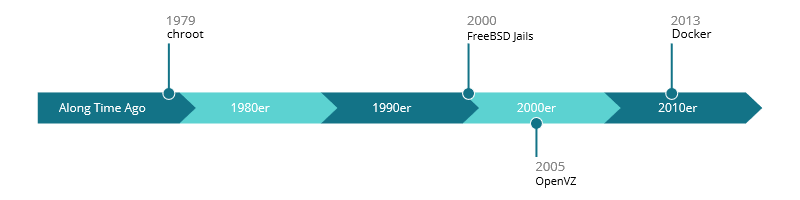
\includegraphics[width=1\textwidth]{ZeitContainer.png}
	\end{center}
	\caption[Containertechnologie im Laufe der Zeit]{Containertechnologie im Laufe der Zeit}
	\label{fig:CTZeit}
\end{figure}


\subsection*{chroot}
\label{sec:chroot}

Chroot ist ein Befehl, der schon früh in Unix-Systemen eingebaut wurde.
Er ermöglicht es einem Prozess, ein anderes Rootverzeichnis zu geben.
Wird in einem Programm \code{chroot()} aufgerufen, wechselt es das Verzeichnis und kann nicht auf Dateien außerhalb der zugewiesenen Struktur zugreifen.
Diese Abschottung eines Prozess war nie als Sicherheitsfeature vorgesehen und wird hauptsächlich zur Virtualisierung eingesetzt.
Mit dem Befehl können einzelne Prozesse auf Dateiebene von anderen Anwendungen getrennt werden, weitere Sicherheitsmechanismen oder Isolierungen gibt es nicht.\cite{IEEE7830207,569694, MANPAGE01}
\newpage
\subsection*{OpenVZ}
\label{sec:OpenVZ}

\begin{wrapfigure}{l}{0.4\textwidth}
	\vspace{-40pt}
	\begin{center}
		
\includegraphics[width=0.3\textwidth]{openvz.png}
	\end{center}
	\vspace{-15pt}
	\caption[Logo OpenVZ]{ \footnotemark}
	\label{fig:openvz}
	\vspace{-30pt}
\end{wrapfigure}
\quellefoot{https://upload.wikimedia.org/wikipedia/commons/b/bb/OpenVZ-logo.png?download}

Im Jahr 2005 veröffentlichte die Firma SWsoft (später umbenannt zu Parallels) ihr Projekt OpenVZ unter der GNU GPL Lizenz. OpenVZ basierte auf der Idee der Container, ermöglicht es jedoch in jedem Container eine eigene Linux-Distribution auszuführen.
Die durch die Containerumgebung abgegrenzten Betriebssysteme, teilen sich dabei einen Kernel. Dadurch ist der Overhead von OpenVZ deutlich geringer als bei der klassischen Vollvirtualisierung eines Betriebssystems.
In den einzelnen Containern gibt es jeweils einen eigenen root-User und eine eigene Dateistruktur.
Sie können unabhängig voneinander gestarten und gestoppt werden.
Da sich die Betriebssysteme einen Kernel teilen, können auch die Gastsysteme nur Linux-Systeme sein.
Da viele der Änderungen von OpenVZ den Kernel von Linux betreffen, werden regelmäßig Änderungen von OpenVZ-Patches in den Kernel von Linux übernommen.\cite{OpenVzNews, IEEE4803091,OpenVzHist}


\subsection*{FreeBSD Jails}
\label{sec:jails}
Mit der Veröffentlicheung von FreeBSD 4.0 im Jahr 2000 war FreeBSD Jails das erste richtige System in der Containervirtualisierung.
Die FreeBSD Jails basieren auf dem Konzept von chroot. Auch hier wird das root-Verzeichnis eines Prozess geändert. Zusätzlich verbessert Jails das Konzept um einige Aspekte, so erhält jede Jail einen eigenen Hostnamen	und eine eigene IP-Adresse. Jede Jail hat auch ihre eigenen Benutzer, inklusive einem root-Benutzer. \cite{FreeBSDHB14} Durch diese Prozessisolation ergibt sich eine Art Containersystem. Da die Jails als eigener Prozess laufen, können sie unabhängig voneinander gestartet und gestoppt werden.  Jails wird gerne für den Einsatz in Netzwerkaufgaben eingesetzt, da die Performance sehr gut ist. Jails besitzt allerdings kein so großes Ökosystem wie Bespielsweise Docker oder OpenVZ. Daher wird es in der Containervirtualisierung von diesen Gegenspielern verdrängt.


\subsection*{\ac{LXC}}
\label{sec:LXC}
\begin{wrapfigure}{r}{0.4\textwidth}
	\vspace{-40pt}
	\begin{center}
		\includegraphics[width=0.3\textwidth]{LXC.png}
	\end{center}
	\vspace{-15pt}
	\caption[Logo \ac{LXC}]{ \footnotemark}
	\label{fig:LXC}
	\vspace{-30pt}
\end{wrapfigure}
\quellefoot{https://upload.wikimedia.org/wikipedia/commons/4/40/Linux_Containers_logo.png?download}
\ac{LXC} ist seit der erstmaligen Veröffentlichung 2008 ein offizielles Kernelfeature und in den meisten Distributionen von Linux enthalten. \ac{LXC} ist eine User Space-Schnittstelle für die erstellung von isolierten Umgebungen innerhalb eines Systems. Dies geschieht durch die Nutzung von Kernel namespace, Apparmor und SELinux-Profilen sowie chroots und cgroups. Diese Features standen schon vor \ac{LXC} zur Verfügung, jedoch vereinigte sie \ac{LXC} zu einer Schnittstelle für die Erzeugung von Containern. Zu Beginn der Entwicklung von \ac{LXC} war die Isolation der Container nicht so gut, sondern glich eher einer Abwandlung der chroot-Funktion. Mit der Zeit wurde die Abschottung jedoch immer besser und die \ac{LXC}-Container wurden zu richtigen virtualisierten Umgebungen. Dies geschah unter anderem dadurch, dass ab Version 1.0 die einzelnen Container als unpriviliegierte Benutzter ausgeführt werden können. Zuvor war dies nicht möglich und eine Abgrenzung der Container nur bedingt gegeben. \ac{LXC} ist eine Technologie, die von vielen weiteren Projekten eingesetzt wird, unter anderen auch Proxmox oder Docker (bis Version 1.1)\cite{IEEE7036275, IEEE7185212, IEEE7571957,IEEE7929714,LXCHomepage}


\subsection*{LXD}
\label{sec:lxd}

Um die Verwendung von \ac{LXC} zu vereinfachen wurde das Tool LXD entwickelt. Es besteht aus drei Elementen: Einem Deamon, der eine REST-API zur Verfügung stellt, einem Befehlszeilenclient sowie einem Open-Stack Nova Plugin. Die vom Deamon bereit gestellte Schnittstelle ermöglicht es, über das Netzwerk auf das Management der Container zuzugreifen. LXD ist somit eine Erweiterung, die eine Schnittstelle zu \ac{LXC}-Containern schafft. Über das Nova Plugin können die einzelnen LXD-Maschinen als Rechenknoten verwendet werden. \cite{LXDHomepage}

\subsection*{Solaris Container}
\label{sec:solariscontainer}

Im Jahr 2004 veröffentlichte Oracle im Build 51 von Solaris 10 zum ersten Mal ein Feature mit dem Namen Solaris Containers. Solaris Container stellt eine Technologie dar, mit der auf x86 und SPARC-Systemen Betriebssystemlevelvirtualisierung durchgeführt werden kann. Später zusammengelegt zu Solaris Zones, bestanden die beiden Technologien Solaris Containers und Solaris Zones parallel zueinander. Dabei war Zones eine klassische Virtualisierungsplatform mit Hypervisor und Containers eine Containertechnologie, die analog zu chroot funktionierte. Mit der Zusammenlegung von Containers und Zones zum neuen Zones wurde daraus eine Containerumgebung, in der die Container sicher voneinander und dem Host getrennt sind und von einem Resourcenmanagement kontrolliert werden.\cite{OracleZonesIntro,OracleZonesOver}
	

%\subsection{Windows Containers}
%s\label{sec:WindowsContainers}



\subsection*{Docker}
\label{sec:Docker}


dotCloud veröffentlichte am März 2013 das Projekt mit dem Namen Docker, dieses Projekt stellte Solomon Hykes auf der PyCon 2013 zum ersten Mal der Öffentlichkeit vor. \cite{dockeryout1} Ein paar Monate Später kündigte dotCloud Inc. an, den Firmennamen zu Docker Inc. zu ändern und sich hauptsächlich der Entwicklung des Docker Ökosystems zu widmen.\cite{dockerblog} Die Firma Docker Inc. (im Folgenden "`Docker Inc."' oder "`Hersteller"') hat bis zum heutigen Tag das Projekt Docker (Im Folgenden "`Docker"') weiterentwickelt und das Ökosystem darum ausgebaut. So wurde unter Anderen der DockerHub eingerichtet, eine Plattform um Images zu teilen und auszutauschen.\cite{dockermanual}

Zu Beginn war Docker lediglich eine Werkzeugsammlung, um \ac{LXC}-Container zu verwalten, jedoch baute Docker Inc. diese Sammlung immer weiter aus und erweiterte das System um Funktionen, die vom unterliegenden Linux-Betriebssystem nicht gegeben waren. Mit der Version 0.9 veröffentlichte Docker Inc. den neuen Treiber libcontainer und nutzte ihn von dort an als native Umgebung für Docker-Container. \cite{dockerblog2} Zu Beginn unterstützte Docker lediglich Linux-Container und nutzte dazu unter Windows eine virtuelle Maschine (Windows 7 \& 8) oder das Linux-Subsystem (Windows 10). Ab der Version 17.11 von Docker für Windows und dem Windows 10 Fall Creators Update konnten erstmals Windows Containers genutzt werden. \cite{dockerblogwin} Auch entwickelte Docker Inc. weitere Zwischebenen, um sich von \ac{LXC} zu lösen und die Umgebung in Module zu teilen. So entstand containerd, ein Container-Deamon, mit dem die Docker Engine kommuniziert. Dieser Deamon wiederum kann mit einem OCI-konformen Container-Tool umgehen und über dieses Container starten. Ein solches Tool ist das eigene runC. Auf diese Art können Docker-Container auch durch andere Orchestrierungstools wie Kubernetes oder Swarm verwaltet werden (\Vgl \Abschnitt{Cluster}).\cite{Buch}

Zum heutigen Zeitpunkt ist Docker die führende Containerumgebung (\Vgl \Abbildung{Stats2}), daher ist die Funktion derselben im Folgenden anhand eines Beispielcontainers aufgezeigt:

In diesem Beispiel soll innerhalb eines Docker-Containers ein python-Skript ausgeführt werden. Zu Beginn eines jeden Containers steht ein Image. Auf diesem schreibgeschützten Image basiert später eine schreibbare Container-Instanz. Ein Image enthält alle benötigten Teile des OS abgesehen vom Kernel, denn dieser wird bereits durch den Host zur Verfügung gestellt. Zusätzlich gehören auch benötigte Anwendungen zu einem Image. Auf diesem schreibgeschützten Teil wird dann ein schreibbarer Layer aufgebaut, wenn von dem Image eine Container-Instanz abgeleitet wird. Wird die Container-Instanz beendet, sind alle Änderung innerhalb des schreibbaren Layer verloren. Um die Änderungen zu sichern kann ein sogenannter Snapshot angelegt werden, der dem Image ein weiteres read-only-Layer hinzufügt. Die Anzahl der Layer ist, je nach Docker-Version auf 127 beschränkt. \cite{Buch, dockermanual} Zum Beispiel könnte ein Image für den Beispielcontainer wie folgt aussehen:

\begin{figure}[h]
    \vspace{-10pt}
    \begin{center}
        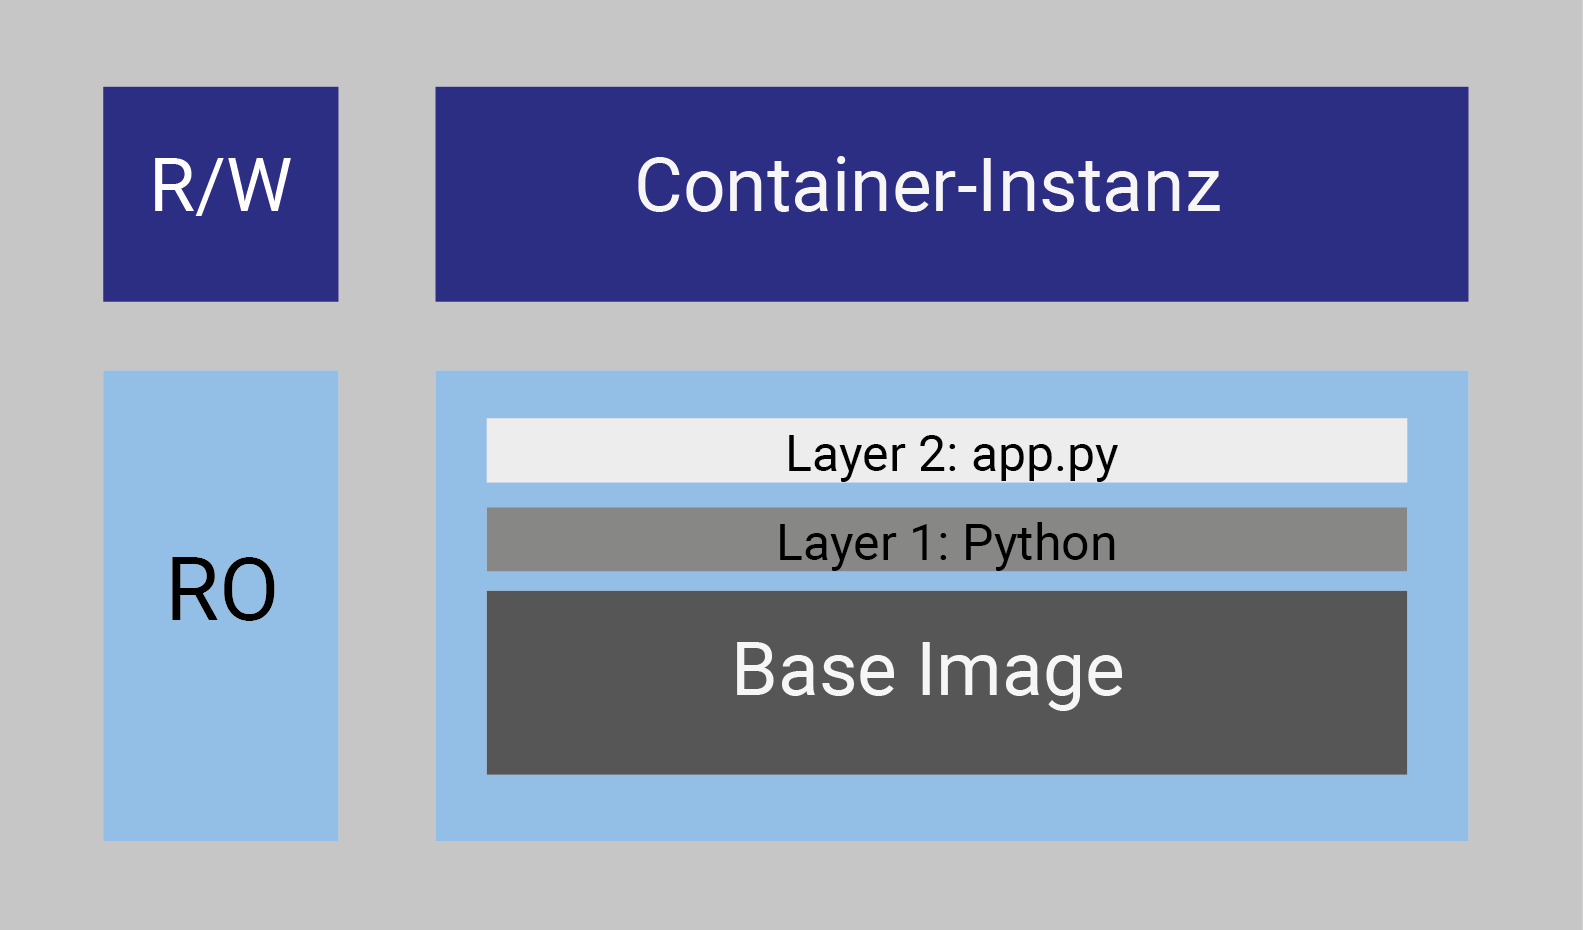
\includegraphics[width=0.6\textwidth]{DockerImage.png}
    \end{center}
    \caption[Image des Beispielcontainer ]{Image des Beispielcontainer}
    \label{fig:docker1}
    \vspace{-10pt}
    \end{figure}

Als Basis dient ein Image, in dem Alpine Linux installiert ist und darauf python. Zu diesen Layern wollen wir noch das python-Skript hinzufügen. Dies ist dann der schreibgeschützte Teil, von dem der Container abgeleitet wird. In dieser Container-Instanz legt das python-Skript dann Dateien an und schreibt in diese. Wird der Container dann beendet, werden alle angelegten Dateien verworfen.\\
Dieses Image kann in einem Dockerfile beschrieben werden. Dies sieht für diesen Fall wie folgt aus:

\begin{lstlisting}[language=docker,label={code:dockerfile}]
    FROM python:3
    
    WORKDIR /usr/src/app
    
    COPY ./app.py ./app.py
    
    CMD ["python", "./app.py"]
\end{lstlisting}

In dem Dockerfile wird zuerst definiert, dass das Image auf vorhanden dem python-Image aufbauen soll. Dieses wiederum baut auf einem Alpine-Linux-Image auf. Daraufhin wird das aktuelle Arbeitsverzeichnis im Container geändert. Dann wird die im Arbeitsverzeichnis des Host abgelegte Datei "`app.py"' in das Arbeitsverzeichnis des Container übertragen und schließlich der Befehl definiert, der beim Starten des Container ausgeführt werden soll. Das Python-Skript legt ein Datei an und gibt deren Dateiname und Inhalt zur Konsole aus:
\begin{lstlisting}[language=python,label={code:pythonapp}]
#!/usr/bin/python3

print("Ausgabe zur Kommandozeile")
file=open("datei.txt", "a+")
print("Dateiname: ", file.name)
file.write("Eine neue Zeile")
file.close()
print(open("datei.txt","r").read())
\end{lstlisting}
Nun kann mit dem Befehl \code{docker build} das Image erstellt werden. Dabei lädt Docker zunächst das Image von python aus dem oben genanten Docker-Hub herunter und legt darauf das Layer mit dem python-Skript:

\begin{lstlisting}[language=bash,label={code:dockerbuild}]
user@dockerpc:~$ docker build -t pythontest .
Sending build context to Docker daemon 311.4MB
Step 1/4 : FROM python:3
 ---> 638817465c7d
Step 2/4 : WORKDIR /usr/src/app
---> 8d3ab23442c9
Step 3/4 : COPY ./app.py ./app.py
---> 2b0882cadee4
Step 4/4 :  CMD ["python", "./app.py"]
---> 5a8a392a0856
Successfully built 5a8a392a0856
Successfully tagged pythontest:latest
\end{lstlisting}

Nun liegt das Image bereit und es kann ein Container davon abgeleitet werden. Dazu reicht nur der einfache Befehl \code{docker run} um den Container zu starten:

\begin{lstlisting}[language=bash,label={code:dockerbuild}]
user@dockerpc:~$ docker run pythontest
Ausgabe zur Kommandozeile
Dateiname: datei.txt
Eine neue Zeile
\end{lstlisting}

Hier wird nun das Python-Skript in dem Container ausgeführt und der Container daraufhin beendet und somit auch die beschriebene Datei gelöscht. Wird der Container erneut ausgeführt, so wird eine neue Datei erstellt:

\begin{lstlisting}[language=bash,label={code:dockerbuild}]
user@dockerpc:~$ docker run pythontest
Ausgabe zur Kommandozeile
Dateiname: datei.txt
Eine neue Zeile

user@dockerpc:~$ docker run pythontest
Ausgabe zur Kommandozeile
Dateiname: datei.txt
Eine neue Zeile
\end{lstlisting}

Die Layer, aus denen Docker die verschiedenen Images aufbaut wurden von Docker Inc. zu dem ursprünglichen \ac{LXC}-Container hinzugefügt und später zum hauseigenen libcontainer übernommen. Durch diese Layer ist es einfacher Ressource zu teilen. Wenn mehrere Images auf Pyhton oder Alpine-Linux aufbauen sollen, so müssen diese beiden Ressourcen nicht mehrfach heruntergeladen werden, sondern können jedem Image zur Verfügung gestellt werden. Dies ist einer der Gründe, warum Docker nach der Veröffentlichung eine große Popularität erreichte und heute die führende Containertechnologie ist.\cite{dockermilestones}



\subsection*{rkt}
\label{sec:rkt}

\begin{wrapfigure}{l}{0.4\textwidth}
	\vspace{-40pt}
	\begin{center}
		
\includegraphics[width=0.3\textwidth]{rkt.png}
	\end{center}
	\vspace{-15pt}
	\caption[Logo rkt]{ \footnotemark}
	\label{fig:rkt}
	\vspace{-30pt}
\end{wrapfigure}
\quellefoot{https://github.com/rkt/rkt/raw/master/logos/rkt-horizontal-color.png}


rkt (Ausprache wie "rocket") ist eine Containerengine, die sich als Alternative zu Docker etabliert und von CoreOS veröffentlicht wurde und weiterentwickelt wird. Das Projekt ist ein Open-Source-Projekt und unter der Apache License 2.0 veröffentlicht.\cite{RepoRkt} Unter rkt werden viele Grundgedanken von UNIX umgesetzt, so liegen alle Container als Dateien vor, die einfach verwaltet werden können. Auch legt rkt einen großen Wert auf Sicherheit und setzt dazu verschiedene Techniken ein, die inzwischen von den meisten Konkurennten übernommen wurden. So kann rkt für jeden Container entscheiden, ob dieser auf Basis von KVM oder einer Virtual Machine isoliert wird und führt alle Prozesse, auch den Download von Images, als nicht priviligierter Benutzer aus. In rkt wird die kleinste Einheit ein "pod" genannt. Sie kann aus einem oder mehrerm Containeren bestehen, die sich Ressourcen teilen. So passt das Konzept von  rkt direkt zu den Konzepten von  Cluster-Managern. Auch besitzt rkt keinen zentralen Service, der alle Container überwacht, sondern arbeitet direkt mit dem Systemeigenen systemd zusammen, um die Container zu verwalten. Somit lässt sich rkt auch direkt mit Kubernetes verknüpfen, für das der Herausgeber von rkt, CoreOS, die kommerzielle Implementierung Tectonic entwickelt. rkt unterstützt auch die Konvertierung von Docker-Containern zu rkt-Pods.\cite{HomepageRkt,ixrkt}

